\section{Results}
\label{sec:results}

\begin{table*}[t]
\centering
\caption{Test-set results on 426 held-out sentences from the 10 training sessions. PER is from greedy CTC decoding. WER is from lexicon-constrained beam search without an LM, with the Kneser--Ney trigram, and after GPT-2 rescoring of the 10-best list. Multi-seed rows are mean\,$\pm$\,s.d.\ over seeds. ``Ensemble'' averages per-frame posteriors over the seeds. GPT-2 rescoring was run only on the best single models; $^\dagger$\,seed 0 only. The Conformer has a single seed (its second seed was stopped for lack of CPU time).}
\label{tab:main}
\begin{tabular}{lcccc}
\toprule
Model & PER & \multicolumn{3}{c}{WER} \\ \cmidrule(lr){2-2}\cmidrule(lr){3-5}
 & greedy & no LM & 3-gram & +GPT-2 \\
\midrule
GRU baseline (published recipe) (2 seeds) & 60.2\,$\pm$\,17.9 & 92.8\,$\pm$\,6.1 & 81.0\,$\pm$\,20.5 & 66.5$^\dagger$ \\
\quad ensemble of 2 & 75.3 & 95.7 & 87.2 & -- \\
GRU + time mask + electrode dropout (2 seeds) & 59.7\,$\pm$\,14.8 & 92.1\,$\pm$\,5.8 & 81.1\,$\pm$\,16.4 & -- \\
\quad ensemble of 2 & 75.7 & 95.3 & 85.9 & -- \\
Causal Conformer + SC-CTC (1 seed) & 38.8 & 83.2 & 52.1 & 51.7 \\
\bottomrule
\end{tabular}
\end{table*}

\begin{figure*}[t]
\centering
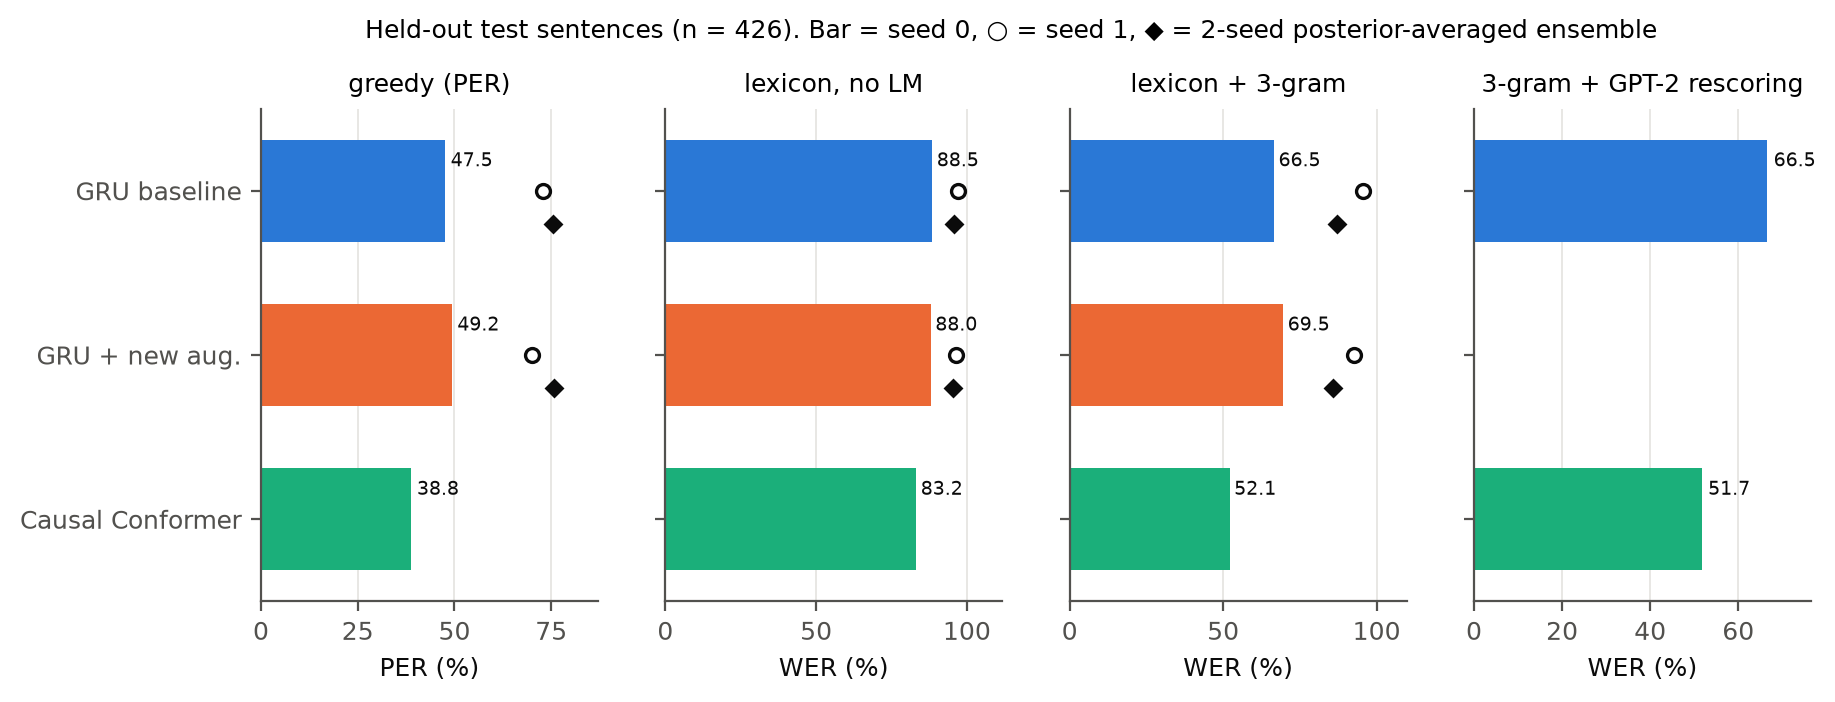
\includegraphics[width=\textwidth]{main_results.png}
\caption{Error rates per model and decoding stage (Table~\ref{tab:main}). Bars show seed~0, open circles seed~1, and diamonds the 2-seed posterior-averaged ensemble. GRU seed~1 stalled in both configurations, and averaging it into an ensemble degrades the converged seed.}
\label{fig:main}
\end{figure*}

\subsection{Neural decoders}
Table~\ref{tab:main} and Fig.~\ref{fig:main} give the main comparison.
The \textbf{causal Conformer} reaches \ConfPER\% PER and \ConfWERng\% WER with the trigram. The best GRU seed reaches \BaseSZeroPER\% PER and \BaseSZeroWERng\% WER (baseline, seed 0).
Its training curve (Fig.~\ref{fig:curves}) has a distinctive shape. For roughly the first 150 steps the Conformer predicts only blanks (dev PER 100\%): the CTC ``blank plateau''. It then improves faster than any GRU and ends below them. Two changes were needed to get there: removing the absolute positional encoding, and using a longer warm-up.
This matches the Brain-to-Text~'24 experience \citep{willett2024b2t}: attention-based encoders are harder to optimize on this data, but they are not intrinsically worse. A practical consequence is that a short pilot run can wrongly rule out a Conformer.

The \textbf{GRU recipe was seed-sensitive} at this budget. With seed~0, both GRU variants train normally (\BaseSZeroPER\% and \AugSZeroPER\% test PER). With seed~1, both stall (\BaseSOnePER\% and \AugSOnePER\%) (Fig.~\ref{fig:curves}, dashed). The mean\,$\pm$\,s.d.\ in Table~\ref{tab:main} reflects this bimodality rather than Gaussian noise. Averaging the posteriors of a converged seed with those of a stalled one is \emph{worse than either member}: \BaseEnsPER\% PER for the baseline ensemble and \AugEnsPER\% for the augmented one (Table~\ref{tab:ablation}). The stalled model's diffuse posteriors corrupt the confident ones. A production pipeline should gate ensemble members on dev PER.

\begin{figure}[t]
\centering
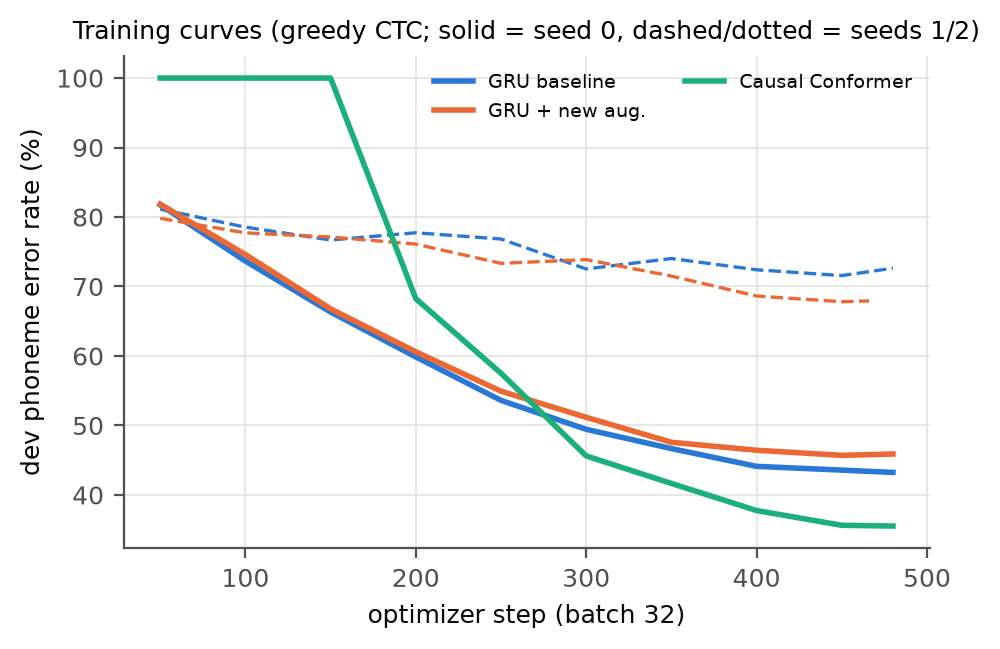
\includegraphics[width=\columnwidth]{training_curves.png}
\caption{Dev PER during training. The Conformer stays on the CTC blank plateau for about 150 steps, then overtakes the GRUs. GRU seed~1 (dashed) stalls for both augmentation settings.}
\label{fig:curves}
\end{figure}

\subsection{Augmentation and day-specific layers}
Table~\ref{tab:ablation} separates the components. \textbf{Time masking and electrode dropout} did \emph{not} improve clean test accuracy at this budget. With seed 0, PER is \AugSZeroPER\% against \BaseSZeroPER\% without them, a difference within the seed noise we observe. This is expected for an under-trained model that is not yet overfitting: regularization pays off when the model is data-limited rather than optimization-limited.
A modest benefit appears under electrode loss (\S\ref{sec:robust}).

\textbf{Day-specific input layers} matter. We evaluated the trained models with the \emph{wrong} day's layer, without retraining. For the GRU, using the previous session's layer raises PER from \SwapAugOwn\% to \SwapAugPrev\%; using the most distant session's layer (up to 4.5 months away) raises it to \SwapAugFar\%; replacing the layer by the identity gives \SwapAugIdent\%.
For the Conformer the corresponding numbers are \SwapConfOwn\%, \SwapConfPrev\%, \SwapConfFar\% and \SwapConfIdent\%. The penalty grows with the time between sessions, as expected from drifting recordings. Even the adjacent session's layer costs 3--6 points, which is why a new day needs calibration (\S\ref{sec:calib}). Interestingly, for the Conformer a distant day's layer is \emph{worse} than no day layer at all.
(We had planned a train-time ablation without day layers, but it did not fit the CPU budget; it is included in \texttt{gpu.yaml}.)

\begin{table}[t]
\centering
\caption{Component analysis. Augmentation: test PER/WER for seeds 0/1. Day layer: test PER when every session is decoded through a different input layer (no retraining), shown as GRU + new aug.\ / Conformer.}
\label{tab:ablation}
\resizebox{\columnwidth}{!}{\begin{tabular}{lcc}
\toprule
Configuration & PER & WER (3-gram) \\
\midrule
\multicolumn{3}{l}{\emph{Augmentation (GRU, per seed: s0 / s1)}} \\
\quad published (noise, offset, cut) & 47.5 / 72.8 & 66.5 / 95.5 \\
\quad + time mask + electrode dropout & 49.2 / 70.1 & 69.5 / 92.7 \\
\multicolumn{3}{l}{\emph{Ensembling (posterior average of s0+s1)}} \\
\quad GRU baseline & 75.3 & 87.2 \\
\quad GRU + new aug. & 75.7 & 85.9 \\
\multicolumn{3}{l}{\emph{Day-specific input layer at test time (PER only)}} \\
\quad own day & 49.2 / 38.8 & -- \\
\quad previous session's layer & 52.1 / 44.7 & -- \\
\quad most distant session's layer & 56.4 / 53.0 & -- \\
\quad identity (no day layer) & 58.1 / 48.5 & -- \\
\quad\footnotesize (GRU + new aug. / Conformer) & & \\
\bottomrule
\end{tabular}}
\end{table}

\subsection{Language-model stack}
\label{sec:lmres}
Table~\ref{tab:lm} shows where the word errors are removed.
Lexicon-constrained decoding without an LM performs poorly: \ConfWERlex\% WER for the Conformer, even though its PER is \ConfPER\%. A PER near 40\% leaves most words with at least one wrong phoneme, and the lexicon alone cannot repair them.
The trigram removes more than a third of the word errors, bringing the Conformer to \ConfWERng\% (bootstrap 95\% CI \ConfNGlo--\ConfNGhi\%).
GPT-2 rescoring of the 10-best list helps only marginally (\ConfWERllm\%, with $\gamma=0.75$ chosen on dev). For the GRU, dev tuning selected $\gamma=0$, so rescoring changes nothing.
The \emph{oracle} over the 10-best list is \ConfOracle\% for the Conformer and \BaseOracle\% for the GRU. With error rates this high, the correct sentence is rarely in the list at all, so no rescorer can help much. Clinical systems rescore from a far stronger starting point.
For this regime, the order of priorities is a better neural decoder first and a better LM second.
The LM's contribution also depends on the material (Fig.~\ref{fig:corpus}). Conversational Switchboard sentences reach \CorpusSwitchboard\% WER, but random word sequences, where the LM can only hurt, reach \CorpusRandom\%.

\begin{figure}[t]
\centering
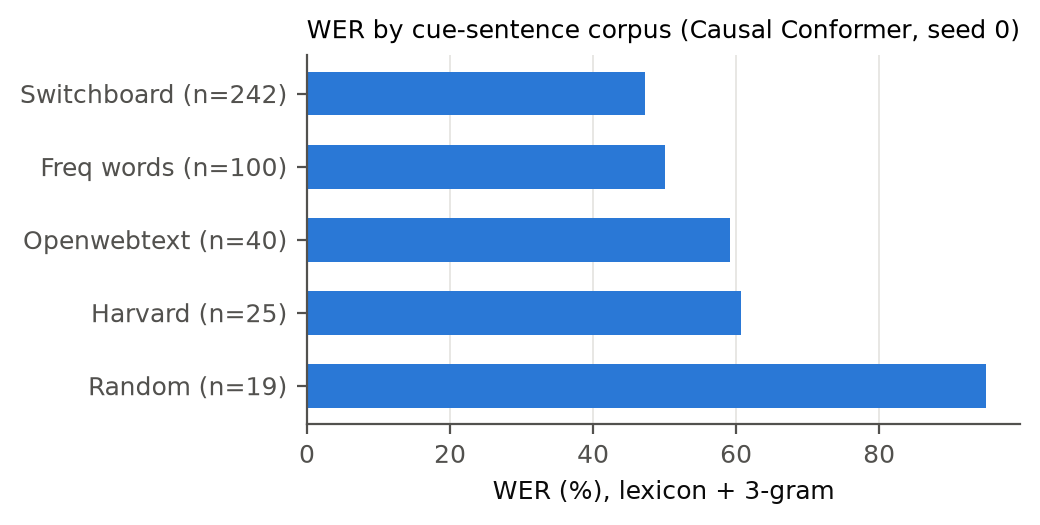
\includegraphics[width=\columnwidth]{wer_by_corpus.png}
\caption{Conformer (seed 0) test WER with the trigram, by cue-sentence corpus.}
\label{fig:corpus}
\end{figure}

\begin{table}[t]
\centering
\caption{WER (\%) at each decoding stage. ``Oracle@10'' is the lowest WER reachable by choosing within the trigram decoder's 10-best list.}
\label{tab:lm}
\resizebox{\columnwidth}{!}{\begin{tabular}{lccccc}
\toprule
System & greedy PER & no LM & 3-gram & +GPT-2 & oracle@10 \\
\midrule
Conformer (s0) & 38.8 & 83.2 & 52.1 & 51.7 & 48.2 \\
GRU baseline (s0) & 47.5 & 88.5 & 66.5 & 66.5 & 63.1 \\
GRU baseline ens. & 75.3 & 95.7 & 87.2 & -- & -- \\
GRU + new aug. ens. & 75.7 & 95.3 & 85.9 & -- & -- \\
\bottomrule
\end{tabular}}
\end{table}

\subsection{Calibration to a new day}
\label{sec:calib}
Figure~\ref{fig:calib} shows what happens on session 2024-03-15, 77 days after the last training session, using the GRU + new aug.\ (s0) model.
Without any new data, reusing the most recent day's layer gives \CalReusePER\% PER and \CalReuseWER\% WER. The same model gets \AugSZeroPER\% PER on in-distribution sessions.
Fine-tuning \emph{only the new day's input layer} on 25 sentences, a few minutes of attempted speech, lowers WER to \CalDayTwentyFiveWER\%. With 200 sentences it reaches \CalDayTwoHundredWER\%.
Fine-tuning \emph{the whole network} on the same sentences is no better from 25 sentences on: \CalFullTwentyFiveWER\% at 25 sentences and \CalFullTwoHundredWER\% at 200. At 10 sentences the two are tied (\CalFullTenWER\% vs.\ \CalDayTenWER\%). It also changes every weight, which is a larger regulatory and safety surface for a medical device than retraining one input layer.
The test set for this day is small (48 sentences), so differences of 2--3 WER points are within noise (bands in Fig.~\ref{fig:calib}).

\begin{figure*}[t]
\centering
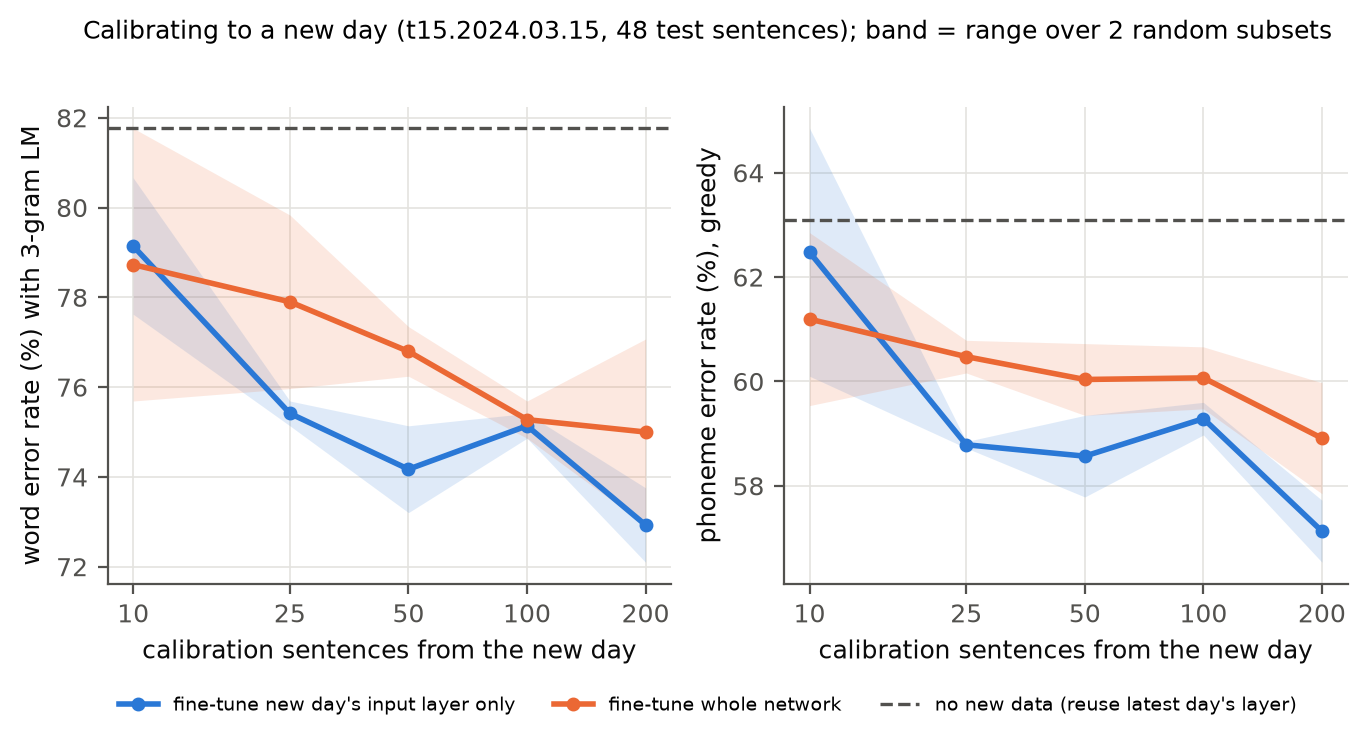
\includegraphics[width=\textwidth]{calibration.png}
\caption{Calibrating to a new day 77 days after training. Day-layer-only fine-tuning recovers most of the attainable improvement within 25 sentences. Full fine-tuning is no better. Bands show the range over two random subsets of calibration sentences.}
\label{fig:calib}
\end{figure*}

\subsection{Robustness to electrode loss}
\label{sec:robust}
Figure~\ref{fig:robust} silences a random fraction of electrodes (both features) at test time, without recalibration.
Silencing 10\% of electrodes costs about one PER point for every model: GRU baseline \RobBaseZero\% $\to$ \RobBaseTen\%, GRU + electrode dropout \RobAugZero\% $\to$ \RobAugTen\%, Conformer \RobConfZero\% $\to$ \RobConfTen\%.
At 50\% loss the GRUs reach \RobBaseFifty\% and \RobAugFifty\%. The model trained with electrode dropout started 1.7 points worse but degraded less, so the gap between the two GRUs has closed. The Conformer degrades the most in absolute terms (to \RobConfFifty\%) but stays the best model at every level of loss.
Decoding is therefore graceful under channel loss: the 512 features are highly redundant for this task. Electrode dropout buys a modest reduction in the slope. Only one random electrode subset was drawn per fraction, so small differences are not significant.

\begin{figure}[t]
\centering
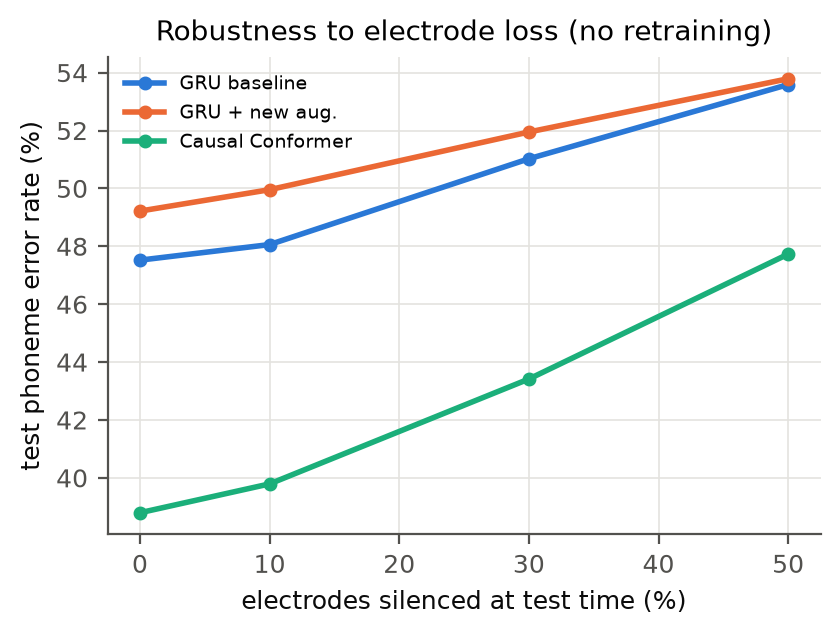
\includegraphics[width=\columnwidth]{robustness.png}
\caption{Test PER when a random subset of electrodes is silenced (one random subset per fraction), with no retraining.}
\label{fig:robust}
\end{figure}

\subsection{Latency and compute}
Table~\ref{tab:latency} reports CPU costs, measured with 2 threads on a heavily shared machine (minimum over 7 repeats, to limit contention effects; absolute values still vary severalfold with load).
The causal GRU costs \LatAugFrame\,ms of compute per 120\,ms output frame when streamed step by step, which is dominated by per-step overhead in PyTorch. The causal Conformer's amortized cost is \LatConfFrame\,ms per frame with a key/value cache. Without a cache, recomputing a 64-frame (7.7\,s) window every frame costs \LatConfRecompute\,ms. That still fits within the 120\,ms frame budget on this CPU, but it wastes about 100$\times$ the cached compute, which matters for power on an implant-class processor.
Both causal models need only the 60\,ms half-width of the smoothing kernel as lookahead. A bidirectional decoder cannot emit anything until the sentence ends.
The language-model stages dominate the latency: \BeamMs\,ms per sentence for our pure-Python beam search and \GPTMs\,ms for GPT-2 rescoring. This argues for streaming word-level beam search (as in WFST decoders) with rescoring only at sentence end.

\begin{table}[t]
\centering
\caption{CPU compute (2 threads) on a median-length test sentence (17\,s). ``Per frame'' is the incremental cost of one 120\,ms output frame. The bidirectional GRU was timed untrained, which does not change its compute.}
\label{tab:latency}
\resizebox{\columnwidth}{!}{\begin{tabular}{lrrrr}
\toprule
Model & params & full fwd & per frame & lookahead \\
 & (M) & (ms) & (ms) & (ms) \\
\midrule
GRU + time mask + electrode dropout & 5.46 & 75 & 2.6 & 60 \\
Bidirectional GRU + new aug. & 8.42 & 161 & -- & sentence \\
Causal Conformer + SC-CTC & 4.99 & 46 & 0.3 & 60 \\
\bottomrule
\end{tabular}}
\end{table}
